% EgoPed architecture figure (TikZ). Grounded in:
%   mld/models/architectures/ego_encoder.py   (EgoEncoder: Linear 2->256, sin. PE, 4x TransformerEncoderLayer, 4 heads, LayerNorm)
%   pretrain_ego_encoder.py                   (mean-pooled ego tokens vs. mean-pooled VAE posterior mean; MSE + 0.1 (1 - cos))
%   mld/models/architectures/mld_denoiser.py  (arch=trans_enc via configs/modules/denoiser.yaml: [z_t | t_emb | c] -> learned PE
%                                              -> 9-layer SkipTransformerEncoder, 4 heads -> first L=4 tokens)
%   mld/models/modeltype/mld.py               (frozen ego encoder; CFG by zeroing the ego input w.p. 0.1; frozen VAE decode)
% Requires: \usepackage{tikz} \usetikzlibrary{arrows.meta,calc,positioning,fit}
\definecolor{ink}{HTML}{1F2A37}
\definecolor{egofill}{HTML}{FAD9A9}\definecolor{egoedge}{HTML}{D48A2A}\definecolor{egotok}{HTML}{EFA54A}
\definecolor{denfill}{HTML}{D4E4F4}\definecolor{denedge}{HTML}{4F82BE}\definecolor{lattok}{HTML}{6E9BD0}
\definecolor{vaefill}{HTML}{EFEFEF}\definecolor{vaeedge}{HTML}{8A8A8A}\definecolor{timetok}{HTML}{BDBDBD}
\definecolor{motfill}{HTML}{CFE6D3}
\begin{tikzpicture}[
  font=\sffamily\scriptsize,
  >={Stealth[length=4pt,width=3.5pt]},
  line/.style={->,draw=ink,line width=0.6pt},
  stage/.style={draw,rounded corners=3pt,line width=0.7pt,align=center,inner sep=3pt,minimum height=11mm},
  enc/.style={stage,fill=egofill,draw=egoedge},
  den/.style={stage,fill=denfill,draw=denedge},
  vae/.style={stage,fill=vaefill,draw=vaeedge,dashed},
  op/.style={draw=ink!70,rounded corners=2pt,line width=0.5pt,fill=white,align=center,inner sep=2.5pt},
  lbl/.style={align=center,inner sep=1pt,text=ink},
  num/.style={circle,draw=ink,fill=white,line width=0.5pt,inner sep=0.6pt,font=\sffamily\tiny\bfseries},
  panel/.style={font=\sffamily\footnotesize\bfseries,anchor=west,inner sep=0pt},
]

% ---------- helpers ----------
% \tokrow{x}{y}{n}{fill}{name}: n adjacent token squares, left edge at x, centred on y
\newcommand{\tokrow}[5]{%
  \foreach \k in {1,...,#3}{%
    \draw[fill=#4,draw=ink,line width=0.35pt] ($(#1,#2)+({(\k-1)*0.2},-0.1)$) rectangle ++(0.2,0.2);}%
  \node[inner sep=0pt,fit={(#1,#2-0.1) ($(#1,#2)+({#3*0.2},0.1)$)}] (#5) {};}
% \grid{x}{y}{cols}{rows}{fill}{name}: small input grid (time along x)
\newcommand{\grid}[6]{%
  \foreach \i in {1,...,#3}{\foreach \j in {1,...,#4}{%
    \draw[fill=#5,draw=ink,line width=0.3pt] ($(#1,#2)+({(\i-1)*0.16},{-(\j-1)*0.16})$) rectangle ++(0.16,-0.16);}}%
  \node[inner sep=0pt,fit={(#1,#2) ($(#1,#2)+({#3*0.16},{-#4*0.16})$)}] (#6) {};}

% =====================================================================
% (a) Ego-encoder pretraining
% =====================================================================
\node[panel] at (0,0.35) {(a) Ego-encoder pretraining};

% row 1: ego trajectory -> ego encoder -> c -> mean-pool
\grid{0.15}{-0.55}{8}{2}{white}{egoA}
\draw[->,ink!70,line width=0.4pt] ($(egoA.north west)+(0,0.12)$) -- ($(egoA.north east)+(0,0.12)$) node[midway,above=-1pt,font=\sffamily\tiny,text=ink!80] {time};
\node[lbl,below=1pt of egoA] {ego trajectory $\mathbf{e}$\\$196\times2$};
\node[enc,minimum width=33mm] (encA) at (4.05,-0.72) {\textbf{Ego encoder}\\Linear $2{\to}256$ + sin.\ PE\\4-layer Transformer, 4 heads};
\node[num] at (encA.north west) {1};
\tokrow{6.25}{-0.72}{8}{egotok}{cA}
\node[lbl,below=1pt of cA] {$\mathbf{c}\in\mathbb{R}^{196\times256}$};
\node[op] (poolA) at (8.85,-0.72) {mean-pool};
\draw[line] (egoA.east) -- (encA.west);
\draw[line] (encA.east) -- (cA.west);
\draw[line] (cA.east) -- (poolA.west);

% row 2: paired motion -> frozen VAE encoder -> mu -> mean-pool
\grid{0.15}{-1.95}{8}{3}{motfill}{motA}
\node[lbl,below=1pt of motA] {paired motion $\mathbf{x}$\\$196\times263$};
\node[vae,minimum width=33mm] (vaeE) at (4.05,-2.2) {\textbf{Motion VAE encoder}\\frozen, posterior mean};
\tokrow{6.25}{-2.2}{4}{lattok}{muA}
\node[lbl,below=1pt of muA] {$\boldsymbol{\mu}\in\mathbb{R}^{4\times256}$};
\node[op] (poolB) at (8.85,-2.2) {mean-pool};
\draw[line] (motA.east) -- (vaeE.west);
\draw[line] (vaeE.east) -- (muA.west);
\draw[line] (muA.east) -- (poolB.west);

% loss
\node[op,minimum width=31mm,minimum height=9mm] (lossA) at (12.35,-1.46)
  {alignment loss in latent space\\[1pt]$\lVert\bar{\mathbf{c}}-\bar{\mathbf{z}}\rVert_2^2+0.1\,\bigl(1-\cos(\bar{\mathbf{c}},\bar{\mathbf{z}})\bigr)$};
\draw[line] (poolA.east) -| node[pos=0.25,above,lbl] {$\bar{\mathbf{c}}\in\mathbb{R}^{256}$} (lossA.north);
\draw[line] (poolB.east) -| node[pos=0.25,below,lbl] {$\bar{\mathbf{z}}\in\mathbb{R}^{256}$} (lossA.south);
\node[lbl,text=ink!75,anchor=west,align=left] at (14.45,-1.46) {gradient reaches\\the ego encoder only};

% =====================================================================
% (b) Diffusion in the VAE latent space
% =====================================================================
\draw[ink!25,line width=0.4pt] (0,-3.35) -- (19.4,-3.35);
\node[panel] at (0,-3.7) {(b) Ego-conditioned latent diffusion (training and DDIM sampling)};

% ego row
\grid{0.15}{-4.35}{8}{2}{white}{egoB}
\node[lbl,below=1pt of egoB] {ego trajectory $\mathbf{e}$\\zeroed w.p.\ 0.1 (CFG)};
\node[enc,minimum width=33mm] (encB) at (4.05,-4.52) {\textbf{Ego encoder}\\frozen, weights from (a)\\no pooling: all 196 tokens};
\node[num] at (encB.north west) {1};
\tokrow{6.25}{-4.52}{8}{egotok}{cB}
\node[lbl,above=1pt of cB] {$\mathbf{c}$: 196 tokens};
\draw[line] (egoB.east) -- (encB.west);
\draw[line] (encB.east) -- (cB.west);

% timestep row
\node[lbl] (tin) at (0.8,-5.75) {timestep $t$};
\node[den,minimum width=33mm,minimum height=7mm] (temb) at (4.05,-5.75) {sinusoidal $+$ MLP};
\tokrow{6.25}{-5.75}{1}{timetok}{tB}
\node[lbl,anchor=west] at ($(tB.east)+(0.05,0)$) {$\mathbf{t}_{\mathrm{emb}}$};
\draw[line] (tin.east) -- (temb.west);
\draw[line] (temb.east) -- (tB.west);

% latent row
\tokrow{6.25}{-6.95}{4}{lattok}{zB}
\node[lbl,above=1pt of zB] {noisy latent $\mathbf{z}_t$: 4 tokens};
\node[lbl,align=left,anchor=west,text=ink!85] (zsrc) at (0.1,-6.95)
  {training: $\mathbf{z}_t=\sqrt{\bar\alpha_t}\,\mathcal{E}(\mathbf{x})+\sqrt{1-\bar\alpha_t}\,\boldsymbol{\epsilon}$\\
   sampling: $\mathbf{z}_T\sim\mathcal{N}(\mathbf{0},\mathbf{I})$};
\draw[line] (zsrc.east) -- (zB.west);

% concatenated sequence  [ z_t (4) | t_emb (1) | c (196) ]
\tokrow{8.15}{-5.75}{4}{lattok}{sZ}
\tokrow{8.95}{-5.75}{1}{timetok}{sT}
\tokrow{9.15}{-5.75}{5}{egotok}{sC}
\node[font=\sffamily\tiny,text=ink] at ($(sC.east)+(0.17,0)$) {\dots};
\node[lbl,above=1pt of sZ] {concatenate};
\node[lbl,below=2pt of sC] {201 tokens\\$+$ learned PE};
\draw[line] (cB.east) -| ($(sC.north)+(0.3,0)$);
\draw[line] (tB.east) ++(0.7,0) -- (sZ.west);
\draw[line] (zB.east) -| (sZ.south);

% denoiser
\node[den,minimum width=29mm,minimum height=17mm] (den) at (12.55,-5.75)
  {\textbf{Transformer denoiser} $\boldsymbol{\epsilon}_\theta$\\9 layers, 4 heads\\self-attention over\\all 201 tokens, long skips};
\node[num] at (den.north west) {2};
\draw[line] ($(sC.east)+(0.35,0)$) -- (den.west);

% read-out
\tokrow{14.55}{-5.75}{4}{lattok}{eps}
\node[lbl,below=1pt of eps] {$\hat{\boldsymbol{\epsilon}}$ = first 4\\output tokens};
\draw[line] (den.east) -- (eps.west);
\node[op] (lossB) at (14.95,-4.5) {training: $\lVert\boldsymbol{\epsilon}-\hat{\boldsymbol{\epsilon}}\rVert_2^2$};
\draw[line,densely dotted] (eps.north) -- (lossB.south);

% DDIM loop and decoding
\node[op] (ddim) at (16.2,-5.75) {DDIM\\update};
\draw[line] (eps.east) -- (ddim.west);
\draw[line] (ddim.south) -- (16.2,-7.95) -| node[pos=0.25,below,lbl] {$\mathbf{z}_{t-1}$, repeated for 50 DDIM steps} (zB.south);
\node[vae,minimum width=13mm,minimum height=8mm,inner sep=2pt] (dec) at (18.0,-5.75) {\textbf{VAE}\\\textbf{decoder}\\frozen};
\draw[line] (ddim.east) -- node[above,lbl] {$\mathbf{z}_0$} (dec.west);
% generated motion, rendered (strip cropped from FINAL_fig1_architecture.png)
\node[inner sep=0pt,anchor=north] (motOut) at ($(dec.south)+(0,-0.3)$)
  {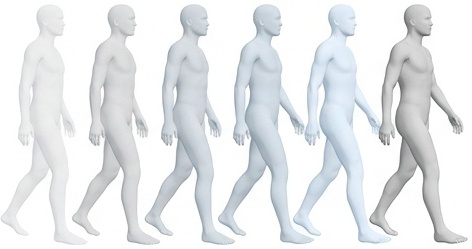
\includegraphics[width=28mm]{figures/architecture_motion.png}};
\draw[line] (dec.south) -- (motOut.north);
\node[lbl,below=1pt of motOut] {generated motion $\hat{\mathbf{x}}$};

% =====================================================================
% legend
% =====================================================================
\begin{scope}[shift={(0,-8.9)},font=\sffamily\scriptsize,
    sw/.style={minimum width=3.5mm,minimum height=2mm,inner sep=0pt,rounded corners=1.5pt,line width=0.5pt},
    tk/.style={minimum size=1.6mm,inner sep=0pt,draw=ink,line width=0.35pt},
    lt/.style={anchor=west,inner sep=1.5pt,text=ink}]
  \node[sw,fill=egofill,draw=egoedge] (l1) at (0.2,0) {};
  \node[lt] (t1) at (l1.east) {pretrained in (a), frozen in (b)};
  \node[sw,fill=denfill,draw=denedge,right=5mm of t1] (l2) {};
  \node[lt] (t2) at (l2.east) {trained in (b)};
  \node[sw,fill=vaefill,draw=vaeedge,dashed,right=5mm of t2] (l3) {};
  \node[lt] (t3) at (l3.east) {pretrained motion VAE, frozen throughout};
  \node[tk,fill=lattok,right=7mm of t3] (l4) {};
  \node[lt] (t4) at (l4.east) {motion latent};
  \node[tk,fill=timetok,right=4mm of t4] (l5) {};
  \node[lt] (t5) at (l5.east) {timestep};
  \node[tk,fill=egotok,right=4mm of t5] (l6) {};
  \node[lt] (t6) at (l6.east) {ego token};
  \node[tk,fill=motfill,right=4mm of t6] (l7) {};
  \node[lt] (t7) at (l7.east) {body motion};
\end{scope}
\end{tikzpicture}
